\scanpage{30}
\uline{isomorphism}, and from which (2) is deduced by passing to the profinite. We thus have a 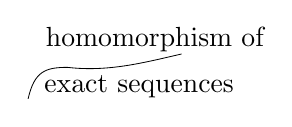
\begin{tikzpicture}[baseline=(base.base)]
\node[anchor=base west,inner sep=0] (base) at (0,0) {exact sequences};
\node[anchor=base west,inner sep=0] at (.02,.58) {\inserted{homomorphism of}};
\draw[line width=.3pt] (-.20,-.08) .. controls (-.12,.27) and (.02,.32) .. (.30,.32) .. controls (.82,.26) and (1.27,.38) .. (1.75,.49);
\end{tikzpicture}
\margin{except if $g=0,\nu=0,1,2$\quad\figure{\begin{tikzpicture}\node[draw,ellipse] {$g=1,\nu=0$};\end{tikzpicture}}?}
\diagram{(4)\quad\begin{tikzcd}[ampersand replacement=\&,column sep=small,row sep=large]
1 \arrow[r,dash] \& \pi_1(\overline M_{g,\nu};\unsure{\xi|j}) \arrow[r,dash] \arrow[d,"\tikz[baseline=-.5ex]{\node[rotate=90,inner sep=0pt] {$\approx$};}"',"\deleted{\unsure{\mathcal T_{g\nu}^{\wedge}}}"] \& \pi_1(M_{g,\nu};\unsure{\xi|j}) \arrow[r] \arrow[d] \& \Gamma \arrow[r,dash] \arrow[d,bend left=20] \& 1\\
1 \arrow[r] \& \mathcal T_{g,\nu}^{\wedge} \arrow[r] \& \operatorname{Autextlac}^{\circ}(\pi_1(X_{\unsure{\xi|j}}\setminus\{x_1,-x_\nu)) \arrow[r] \& \operatorname{Out}\unsure{T} \arrow[d,phantom,"\unsure{\vert|\downarrow}" description]\\
\&\&\&1
\end{tikzcd}}
\unsure{let us assume} that $\mathcal T_{g,\nu}^{\wedge}\unsure{\to|\text{is}}$
\unsure{invariant|injective} in $\operatorname{Autextlac}^{\circ}(\ ?\ )$.
\margin{Possible corrected version: $\pi_1(M_{g,\nu};\unsure{\xi|j})\simeq$ Normalizer of $\mathcal T_{g,\nu}^{\wedge}$ in $\operatorname{Autextlac}^{\circ}(\pi_1(X_{\unsure{\xi|j}}\setminus\{x_1-x_\nu\unsure{\})|\}))}$ inducing \unsure{automorphisms} of $\mathcal T_{g,\nu}^{\wedge}$ commuting with $\mathfrak S_\nu$ and preserving a possible
\figure{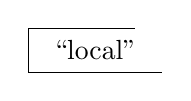
\begin{tikzpicture}
\node[inner sep=1pt] (loc) at (0,0) {``local''};
\draw (-.85,.28)--(-.85,-.28)--(.85,-.28);
\draw (-.85,.28)--(.5,.28);
\end{tikzpicture}}
structure\ldots $*$
\figure{\begin{tikzpicture}\draw (0,0)--(3.7,0);\end{tikzpicture}}}

We \deleted{\unsure{have}} would like the arrow (1) (the central vertical arrow of (5)) to be an \uline{isomorphism}. This would give a characterization of $\Gamma$ as
\[
\operatorname{Autextlac}^{\circ}\left(\pi_1\underbrace{(X^{an}\setminus\{x_1,-x_\nu\})^{\wedge}}_{\substack{\text{standard group}\\\text{well known}}}\right)/\mathcal T_{g,\nu}^{\wedge}
\]
\margin{For $(g,\nu)$ except $g=0,\nu=0,1,2$\quad $g=1,\nu=0$ (case where $\pi_1(X_{\unsure{\overline{\mathbf Q}|\mathbf Q}}\setminus S_\nu)$ \unsure{is a group|is a group} that is abelian).
\figure{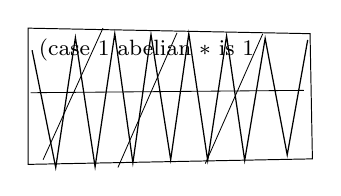
\begin{tikzpicture}
\node[anchor=north west,align=left,text width=3.4cm,font=\footnotesize,inner sep=0] at (0,.85) {\deleted{\unsure{(case} \illegible{1} \unsure{abelian} $*$ \unsure{is} \illegible{1}}};
\draw[line width=.35pt] (-.13,-.75)--(-.13,.98)--(3.45,.91)--(3.48,-.68)--cycle;
\draw[line width=.45pt] (-.08,.70)--(.22,-.79)--(.47,.86)--(.72,-.78)--(.97,.91)--(1.20,-.73)--(1.43,.90)--(1.68,-.69)--(1.91,.91)--(2.15,-.70)--(2.39,.88)--(2.62,-.70)--(2.88,.85)--(3.16,-.63)--(3.42,.83);
\draw[line width=.3pt] (.06,-.69)--(.82,.98) (1.01,-.79)--(1.76,.92) (2.12,-.74)--(2.85,.91) (-.10,.16)--(3.37,.19);
\end{tikzpicture}}}
\margin{For the case $g=0,\nu=3$, it is also advisable to be cautious and to require commutation conditions with the outer \unsure{action|action} of $\mathfrak S_3$\ldots}

\uline{Example} For $g=0,\nu=3$ this would give the expression already envisaged of $\Gamma$ as
\[
\operatorname{Autextlac}^{\circ}(\pi_1(\mathbf P^1\setminus\{0,1,\infty\}).
\]
\mspage{29}
